
\section{Glossary of Symbols}

\begin{table*}[h]
\centering
\begin{tabular}{l l}
\toprule
Symbol & Used for \\
\midrule
$x$, $y$, $z$ & vectors in the Poincar{\'e} ball model of hyperbolic space \\
$d_H$ & metric distance between two points in hyperbolic space \\
$d_E$ & metric distance between two points in Euclidean space \\
$d_U$ & metric distance between two points in metric space $U$ \\
$d$ & a particular distance value \\
$d_{i,j}$ & the distance between the $i$th and $j$th points in an embedding \\
$\mathbb{H}_r$ & the Poincar{\'e} ball model of $r$-dimensional Hyperbolic space \\
$r$ & the dimension of a Hyperbolic space \\
$\mathbb{H}$ & Hyperbolic space of an unspecified or arbitrary dimension \\
$\mathbb{M}_r$ & the Minkowski (hyperboloid) model of $r$-dimensional Hyperbolic space \\
$f$ & an embedding \\
$\mathcal{N}_a$ & neighborhood around node $a$ in a graph \\
$R_{a,b}$ & the smallest set of closest points to node $a$ in an embedding $f$ that contains node $b$ \\
$\text{MAP}(f)$ & the mean average precision fidelity measure of the embedding $f$ \\
$D(f)$ & the distortion fidelity measure of the embedding $f$ \\
$D_{\mathrm{wc}}(f)$ & the worst-case distortion fidelity measure of the embedding $f$ \\
$G$ & a graph, typically with node set $V$ and edge set $E$ \\
$T$ & a tree \\
$a, b, c$ & nodes in a graph or tree \\
$\operatorname{deg}(a)$ & the degree of node $a$ \\
$\operatorname{deg}_{\max}$ & maximum degree of a node in a graph \\
$\ell$ & the longest path length in a graph \\
$\tau$ & the scaling factor of an embedding \\
$\operatorname{reflect}_{x \rightarrow y}$ & a reflection of $x$ onto $y$ in hyperbolic space \\
$\operatorname{arg}(z)$ & the angle that the point $z$ in the plane makes with the $x$-axis \\
$X$ & matrix of points in hyperbolic space \\
$Y$ & matrix of transformed distances \\
% $S$ & diagonal scaling matrix used in h-MDS \\
% $v$ & vector of squared norm values used in h-MDS \\
% $u, \hat u$ & eigenvectors used in h-MDS \\
% $Z$ & reduced matrix used in h-MDS \\
% $\alpha, \beta$ & intermediate scalars used in h-MDS \\
$\gamma$ & geodesic used in PGA \\
$w_i$ & transformed points used in PGA \\
\bottomrule
\end{tabular}
\caption{Glossary of variables and symbols used in this paper.}
\label{table:glossary}
\end{table*}

\section{Related Work}
\label{sec:related}
Our study of representation tradeoffs for hyperbolic embeddings was motivated by
exciting recent approaches towards such embeddings in \citet{fb} and
\citet{ucl}.
Earlier efforts proposed using hyperbolic spaces for routing, starting with Kleinberg's work on geographic routing \cite{Kleinberg}.
\citet{Crovella} performed hyperbolic embeddings and routing for dynamic networks.
Recognizing that the use of hyperbolic space for routing required a large number of bits to store the vertex coordinates, \citet{Eppstein} introduced a scheme for succinct embedding and routing in the hyperbolic plane.
Another very recent effort also proposes using hyperbolic cones (similar to the cones that are the fundamental building block used in \citet{sarkar} and our work) as a heuristic for embedding entailment relations, i.e. directed acyclic graphs~\cite{ganea}.
The authors also propose to optimize on the hyperbolic manifold using its exponential map, as opposed to our approach of finding a closed form for the embedding should it exist (Section~\ref{sec:MDS}). An interesting avenue for future work is to compare both optimization methods empirically and theoretically, i.e., to understand the types of recovery guarantees under noise that such methods have.

There have been previous efforts to perform multidimensional scaling in hyperbolic space (the h-MDS problem), often in the context of visualization~\cite{lamping1994laying}. Most propose descent methods in hyperbolic space (e.g.~\cite{cvetkovski2016multidimensional}, \cite{walter2004}) and fundamentally differ from ours.
Arguably the most relevant is~\citet{wilson2014spherical}, which mentions exact recovery as an intermediate result, but ultimately suggests a heuristic optimization.
Our h-MDS analysis characterizes the recovered embedding and manifold and obtains the correctly centered one---a key issue in MDS.
For example, this allows us to properly find the components of maximal variation.
Furthermore, we discuss robustness to noise and produce optimization guarantees when a perfect embedding doesn't exist.

Several papers have studied the notion of hyperbolicity of networks, starting with the seminal work on hyperbolic graphs \citet{Gromov}. More recently, \citet{Mahoney} considered the hyperbolicity of small world graphs and tree-like random graphs. \citet{Dragan} performed a survey that examines how well real-world networks can be approximated by trees using a variety of tree measures and tree embedding algorithms. To motivate their study of tree metrics, \citet{Abraham} computed a measure of tree likeness on a Internet infrastructure network. 

We use matrix completion (closure) to perform embeddings with incomplete data. Matrix completion is a celebrated problem. \citet{TaoMatrix} derive bounds on the minimum number of entries needed for completion for a 
fixed rank matrix; they also introduce a convex program for matrix completion operating at near the optimal rate.

Principal geodesic analysis (PGA) generalizes principal components analysis (PCA) for the manifold setting. It was introduced and applied to shape analysis in \cite{PGA} and extended to a probabilistic setting in \cite{ProbPGA}.
There are other variants; the geodesic principal components analysis (GPCA) of~\citet{GPCA} uses our loss function.



\section{Low-Level Formulation Details}
We plan to release our PyTorch code, high precision solver, and other
routines on Github. A few comments are helpful to understand the
reformulation. In particular, we simply minimize the squared
hyperbolic distance with a learned scale parameter, $\tau$, e.g., :
\[ \min_{x_1,\dots,x_n,\tau}\sum_{1 \leq i < j \leq n} \left(\tau d_{H}(x_i,x_j) - d_{i,j}\right)^2 \]
We typically require that $\tau \geq 0.1$.

\begin{itemize}
\item On continuity of the derivative of the loss: Note that
  \[ \partial_{x} \mathsf{acosh}(1+x) = \frac{1}{\sqrt{(1+x)^2 -1 }}
= \frac{1}{\sqrt{x(x+2)}} \text{ hence } \lim_{x \to 0} \partial_{x}
\mathsf{acosh}(1+x) = \infty. \] Thus, $\lim_{y \to x} \partial_{x}
d_{H}(x,y) = \infty$. In particular, if two points happen to get near
to one another during execution, gradient-based optimization becomes
unstable. Note that $\exp\{\mathrm{acosh(1+x)}\}$ suffers from a
similar issue, and is used in both~\cite{fb, ucl}. This change may
increase numerical instability, and the public code for these
approaches does indeed take steps like masking out updates to mitigate
\textsc{NaN}s. In contrast, the following may be more stable:
\[ \partial_{x} \mathsf{acosh}(1+x)^2 = 2 \frac{\mathsf{acosh}(1+x)}{\sqrt{x(x+2)}} \text{ and in particular } \lim_{x \to 0} \partial_{x} \mathsf{acosh}(1+x)^2 = 2\]
The limits follows by simply applying L'Hopital's rule. In turn, this
implies the square formulation is continuously differentiable. Note
that it is not convex.
  \item One challenge is to make sure the gradient computed by PyTorch
    has the appropriate curvature correction (the Riemannian metric),
    as is well explained by \citet{fb}. The modification is
    straightforward: we create a subclass of \textsc{nn.Parameter}
    called \textsc{Hyperbolic\_Parameter}. This wrapper class allows
    us to walk the tree to apply the appropriate correction to the
    metric (which amounts to multiplying $\nabla_{w} f(w)$ by
    $\frac{1}{4}(1-\|w\|^2)^2$. After calling the \textsc{backward}
    function, we call a routine to walk the autodiff tree to find such
    parameters and correct them. This allows
    \textsc{Hyperbolic\_Parameter} and traditional parameters to be
    freely mixed.

    \item We project back on the hypercube following \citet{fb} and
      use gradient clipping with bounds of $[-10^{5},10^5]$. This
      allows larger batch sizes to more fully utilize the GPU.
\end{itemize}

\section{Combinatorial Construction Proofs}
\label{app:CombinatorialProofs}

\paragraph{Precision vs. model}

We first provide a simple justification of the fact (used in Section~\ref{sec:sarkar}) that representing distances $d$ requires about $d$ bits in hyperbolic space -- independent of the model of the space.
Formally, we show that the number of bits needed to represent a space depends only on the maximal and minimal desired distances and the geometry of the space.
Thus although the bulk of our results are presented in the Poincar{\'e} sphere, our discussion on precision tradeoffs is fundamental to hyperbolic space.

A representation using $b$ bits can distinguish $2^b$ distinct points in a space $S$.
Suppose we wish to capture distances up to $d$ with error tolerance $\varepsilon$ -- concretely, say every point in the ball $B(0,d)$ must be within distance $\varepsilon$ of a represented point.
By a sphere covering argument, this requires at least $\frac{V_S(d)}{V_S(\varepsilon)}$ points to be represented, where $V_S(r)$ is the volume of a ball of radius $r$ in the geometry.
Thus at least $b=\log \frac{V_S(d)}{V_S(\varepsilon)}$ bits are needed for the representation.
Notice that $V_E(d) \sim d^n$ in Euclidean $\R^n$ space, so this gives the correct bit complexity of $n \log(d/\varepsilon)$.
In hyperbolic space, $V_H$ is exponential instead of polynomial in $d$, so $O(d)$ bits are needed in the representation (for any constant tolerance).
In particular, this is independent of the model of the space.


\paragraph{Graph embedding lower bound}

Now, we derive a lower bound on the bits of precision required for embedding a graph into $\mathbb{H}_2$.
Afterwards we prove a result bounding the precision for our extension of Sarkar's construction for the $r$-dimensional Poincar\'{e} ball $\mathbb{H}_r$. Finally, we give some details on the algorithm for this extension.

We derive the lower bound by exhibiting an explicit graph and lower bounding the precision needed to represent its nodes (for any embedding of the graph into $\mathbb{H}_2$). The explicit graph $G_m$ we consider consists of a root node with $\text{deg}_{\max}$ chains attached to it. Each of these chains has $m$ nodes for a total of $1+m(\text{deg}_{\max})$ nodes, as shown in Figure~\ref{fig:chains}.

\begin{figure}
\centering
\begin{minipage}[b]{0.4\textwidth}
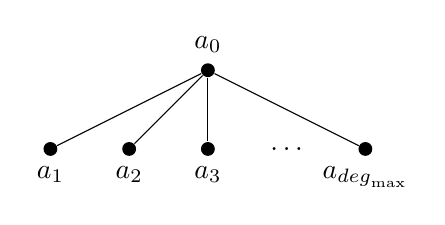
\begin{tikzpicture}[scale=1.0]
\node [circle,fill,inner sep=0pt,minimum size=5pt] (a0) at (0,1) [label={above:$a_0$}]{};
\node [circle,fill,inner sep=0pt,minimum size=5pt] (a1) at (-2,0) [label={below:$a_1$}]{};
\node [circle,fill,inner sep=0pt,minimum size=5pt] (a2) at (-1,0) [label={below:$a_2$}]{};
\node [circle,fill,inner sep=0pt,minimum size=5pt] (a3) at (0,0) [label={below:$a_3$}]{};    
\node [] (dots) at (1,0) [label={center:$\ldots$}]{};    
\node [circle,fill,inner sep=0pt,minimum size=5pt] (a4) at (2,0) [label={below:$a_{\text{deg}_{\max}}$}]{};

\draw (a0) -- (a1);
\draw (a0) -- (a2);
\draw (a0) -- (a3);
\draw (a0) -- (a4);

\end{tikzpicture}
  \end{minipage}
%  \hfill
  \begin{minipage}[b]{0.4\textwidth}
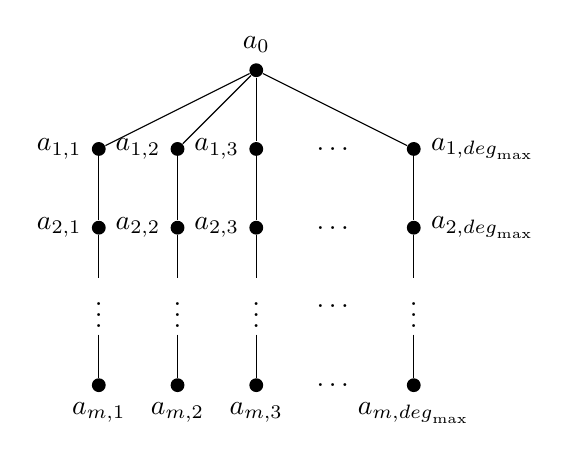
\begin{tikzpicture}[scale=1.0]
\node [circle,fill,inner sep=0pt,minimum size=5pt] (a0) at (0,1) [label={above:$a_0$}]{};
\node [circle,fill,inner sep=0pt,minimum size=5pt] (a1) at (-2,0) [label={left:$a_{1,1}$}]{};
\node [circle,fill,inner sep=0pt,minimum size=5pt] (a2) at (-1,0) [label={left:$a_{1,2}$}]{};
\node [circle,fill,inner sep=0pt,minimum size=5pt] (a3) at (0,0) [label={left:$a_{1,3}$}]{};    
\node [] (dots) at (1,0) [label={center:\ldots}]{};    
\node [circle,fill,inner sep=0pt,minimum size=5pt] (a4) at (2,0) [label={right:$a_{1,\text{deg}_{\max}}$}]{};

\node [circle,fill,inner sep=0pt,minimum size=5pt] (a5) at (-2,-1) [label={left:$a_{2,1}$}]{};
\node [circle,fill,inner sep=0pt,minimum size=5pt] (a6) at (-1,-1) [label={left:$a_{2,2}$}]{};
\node [circle,fill,inner sep=0pt,minimum size=5pt] (a7) at (0,-1) [label={left:$a_{2,3}$}]{};    
\node [] (dots2) at (1,-1) [label={center:\ldots}]{};    
\node [circle,fill,inner sep=0pt,minimum size=5pt] (a8) at (2,-1) [label={right:$a_{2,\text{deg}_{\max}}$}]{};

\node [circle,fill,inner sep=0pt,minimum size=20pt,color=white] (vdots1) at (-2,-2) [label={center:$\vdots$}]{};
\node [circle,fill,inner sep=0pt,minimum size=20pt,color=white] (vdots2) at (-1,-2) [label={center:$\vdots$}]{};
\node [circle,fill,inner sep=0pt,minimum size=20pt,color=white]  (vdots3) at (0,-2) [label={center:$\vdots$}]{};
\node [] (dots2) at (1,-2) [label={center:\ldots}]{};    
\node [circle,fill,inner sep=0pt,minimum size=20pt,color=white]  (vdots4) at (2,-2) [label={center:$\vdots$}]{};

\node [circle,fill,inner sep=0pt,minimum size=5pt] (a9) at (-2,-3) [label={below:$a_{m,1}$}]{};
\node [circle,fill,inner sep=0pt,minimum size=5pt] (a10) at (-1,-3) [label={below:$a_{m,2}$}]{};
\node [circle,fill,inner sep=0pt,minimum size=5pt] (a11) at (0,-3) [label={below:$a_{m,3}$}]{};    
\node [] (dots3) at (1,-3) [label={center:\ldots}]{};    
\node [circle,fill,inner sep=0pt,minimum size=5pt] (a12) at (2,-3) [label={below:$a_{m,\text{deg}_{\max}}$}]{};

\draw (a0) -- (a1);
\draw (a0) -- (a2);
\draw (a0) -- (a3);
\draw (a0) -- (a4);

\draw (a1) -- (a5);
\draw (a2) -- (a6);
\draw (a3) -- (a7);
\draw (a4) -- (a8);

\draw (a5) -- (vdots1);
\draw (a6) -- (vdots2);
\draw (a7) -- (vdots3);
\draw (a8) -- (vdots4);

\draw (vdots1) -- (a9);
\draw (vdots2) -- (a10);
\draw (vdots3) -- (a11);
\draw (vdots4) -- (a12);
    
\end{tikzpicture}
  \end{minipage}
\caption{Explicit graphs $G_m$ used to derive precision lower bound. Left: $m=1$ case (star graph). Right: $m>1$.}
\label{fig:chains}
\end{figure}

\begin{lemma}
The bits of precision needed to embed a graph with longest path $\ell$ is $\Omega\left(\frac{\ell}{\varepsilon} \log(\operatorname{deg}_{\max}) \right)$.
\end{lemma}
\begin{proof}



We first consider the case where $m=1$. Then $G_1$ is a star with $1+\text{deg}_{\max}$ children $a_1, a_2, \ldots, a_{\text{deg}_{\max}}$. Without loss of generality, we can place the root $a_0$ at the origin $0$. 

Let $x_i = f(a_i)$ be the embedding into $\mathbb{H}_2$ for vertex $a_i$ for $0 \leq i \leq \text{deg}_{\max}$.
We begin by showing that the distortion does not increase if we equalize the distances between the origin and each child $x_i$.
Let us write $\ell_{\max} = \max_i d_H(0,x_i) $ and $\ell_{\min} = \min_i  d_H(0,x_i)$. 

What is the worst-case distortion? We must consider the maximal expansion and the maximal contraction of graph distances.
Our graph distances are either 1 or 2, corresponding to edges ($a_0$ to $a_i$) and paths of length 2 ($a_i$ to $a_0$ to $a_j$).
By triangle inequality, $\frac{d_H(x_i,x_j)}{2} \leq \frac{d_H(0, x_i)}{2}+ \frac{d_H(0, x_j)}{2} \leq \ell_{\max}$.
This implies that the maximal expansion $\max_{i \neq j} d_H(f(a_i),f(a_j))/d_G(a_i,a_j)$ is $\frac{\ell_{\max}}{1} = \ell_{\max}$ occuring at a parent-child edge.
Similarly, the maximal contraction is at least $\frac{1}{\ell_{\min}}$. With this,
\[D_{\text{wc}}(f) \geq \frac{\ell_{\max}}{\ell_{\min}}.\]
Equalizing the origin-to-child distances (that is, taking $\ell_{\max} = \ell_{\min}$) reduces the distortion. Moreover, these distances are a function of the norms $\|x_i\|$, so we set $\|x_i\| = v$ for each child. 

Next, observe that since there are $\text{deg}_{\max}$ children to place, there exists a pair of children $x,y$ so that the angle formed by $x,0,y$ is no larger than $\theta = \frac{2\pi}{\text{deg}_{\max}}$. In order to get a worst-case distortion of $1+\varepsilon$, we need the product of the maximum expansion and maximum contraction to be no more than $1+\varepsilon$. The maximum expansion is simply $d_H(0,x)$ while the maximum contraction is $\frac{2}{d_H(x,y)}$, so we wan
\[2d_H(0,x) \leq (1+\varepsilon) d_H(x,y).\]

We use the log-based expressions for hyperbolic distance:
\[d_H(0,x) = \log \left(\frac{1+v}{1-v} \right),\]

and
\begin{align*}
d_H(x,y) &= 2 \log \left( \frac{\|x-y\| + \sqrt{\|x\|^2\|y\|^2 -2\langle x,y \rangle + 1}}{\sqrt{(1-\|x\|^2)(1-\|y\|^2)}} \right) \\
&=2 \log \left(\frac{\sqrt{2v^2(1-\cos \theta)} + \sqrt{v^4-2v^2 \cos \theta + 1}}{1-v^2} \right).
\end{align*}

This leaves us with 
\[  \log \left(\frac{\sqrt{2v^2(1-\cos \theta)} + \sqrt{v^4-2v^2 \cos \theta + 1}}{1-v^2} \right) (1+\varepsilon) \geq \log \left(\frac{1+v}{1-v} \right).\]

Now, since $1 > v^2$, we have that $\sqrt{2(1-\cos \theta)} \geq\sqrt{2v^2(1-\cos \theta)}$. Some algebra shows that  $\sqrt{3(1-\cos \theta)} \geq\sqrt{v^4 - 2v^2\cos \theta + 1}$, so that we can upper bound the left-hand side to write 
\[  \log \left(\frac{(1+\sqrt{\frac{3}{2}}) \sqrt{2(1-\cos \theta)}}{1-v^2} \right) (1+\varepsilon) \geq \log \left(\frac{1+v}{1-v} \right) .\]

Next we use the small angle approximation $\cos(\theta) = 1-\theta^2/2$ to get $\sqrt{2(1-\cos \theta)} = \theta$. Now we have
\[  \log \left(\frac{(1+\sqrt{\frac{3}{2}})  \theta }{1-v^2} \right) (1+\varepsilon) \geq \log \left(\frac{1+v}{1-v} \right) .\]

Since $v < 1$, $\frac{1}{1-v} > \frac{1}{1-v^2}$ and $\frac{1+v}{1-v} \geq \frac{1}{1-v}$, so we can upper bound the left-hand side and lower bound the right-hand side:
\[  \log \left(\frac{(1+\sqrt{\frac{3}{2}})  \theta }{1-v} \right) (1+\varepsilon) \geq  \log \left(\frac{1}{1-v} \right).\]

Rearranging,
\[ -\log(1-v) \geq -\log\left( \left(1+\sqrt{\frac{3}{2}}\right) \theta\right) \frac{1+\varepsilon}{\varepsilon}.\]

Recall that $\theta = \frac{2\pi}{\text{deg}_{\max}}$. Then we have that
\[-\log(1-v) \geq \left(\frac{1+\varepsilon}{\varepsilon} \right) \left(\log (\text{deg}_{\max}) - \log((2+\sqrt{6})\pi) \right),\]
so that
\[-\log(1-v) = \Omega\left(\frac{1}{\varepsilon} \log (\text{deg}_{\max}) \right).\]

Since $v = \|x\| = \|y\|$, $-\log(1-v)$ is precisely the required number of bits of precision, so we have our lower bound for the $m=1$ case. 

Next we analyze the $m>1$ case. Consider the embedded vertices $x_1, x_2, \ldots, x_m$ corresponding to one chain and $y_1, y_2, \ldots, y_m$ corresponding to another. There exists a pair of chains such that the angle formed by $x_m, 0, y_1$ is at most $\theta = \frac{2\pi}{\text{deg}_{\max}}$. Let $u = \|x_m\|$ and $v = \|y_1\|$. From the $m=1$ case, we have a lower bound on $-\log(1-v)$; we will now lower bound $-\log(1-u)$. The worst-case distortion we consider uses the contraction given by the path $x_m \rightarrow x_{m-1} \rightarrow \cdots \rightarrow x_1 \rightarrow 0 \rightarrow y_1$; this path has length $m+1$. The expansion is just the edge between $0$ and $y_1$. Then, to satisfy the worst-case distortion $1+\varepsilon$, we need
\[(m+1)d_H(0,y_1) \leq (1+\varepsilon)d_H(x_m,y_1).\]

Using the hyperbolic distance formulas, we can rewrite this as 
\[ 2 \log \left( \frac{\|x_m-y_1\| + \sqrt{\|x_m\|^2\|y_1\|^2 -2\langle x_m,y_1 \rangle + 1}}{\sqrt{(1-\|x_m\|^2)(1-\|y_1\|^2)}} \right) (1+\varepsilon) \geq (m+1) \log \left(\frac{1+v}{1-v} \right),\]

or,
\[ 2 \log \left( \frac{ \sqrt{u^2+v^2-2uv\cos \theta} + \sqrt{u^2v^2-2uv\cos\theta + 1}}{\sqrt{(1-u^2)(1-v^2)}} \right) (1+\varepsilon) \geq (m+1) \log \left(\frac{1+v}{1-v} \right).\]

Next,
\begin{align*}
2 \log &\left( \frac{ \sqrt{u^2+v^2-2uv\cos \theta} + \sqrt{u^2v^2-2uv\cos\theta + 1}}{\sqrt{(1-u^2)(1-v^2)}} \right) \\
 &\leq 2 \log \left( \frac{(1+\sqrt{\frac{3}{2}})\theta}{\sqrt{(1-u^2)(1-v^2)}} \right) =  \log \left( \frac{(1+\sqrt{\frac{3}{2}})^2\theta^2}{(1-u^2)(1-v^2)} \right) \\
&\leq  \log \left( \frac{(1+\sqrt{\frac{3}{2}})^2\theta^2}{(1-u)(1-v)} \right).
\end{align*}
In the first step, we used the same arguments as earlier. Applying this result and using $\frac{1+v}{1-v} \geq \frac{1}{1-v}$, we have
\[   \log \left( \frac{(1+\sqrt{\frac{3}{2}})^2\theta^2}{(1-u)(1-v)} \right)(1+\varepsilon) \geq (m+1) \log \left(\frac{1}{1-v} \right),\]
or,
\[   \log \left( \frac{(1+\sqrt{\frac{3}{2}})^2\theta^2}{1-u} \right)(1+\varepsilon) \geq (m-\varepsilon) \log \left(\frac{1}{1-v} \right).\]

Next we can apply the bound on $-\log(1-v)$.
\begin{align*}
\log\left(\frac{1}{1-u}\right) &\geq -\log\left((1+\sqrt{\frac{3}{2}})^2\theta^2\right) + \left( \frac{m-\varepsilon}{1+\varepsilon} \right) \log \left(\frac{1}{1-v} \right) \\
&\geq  -\log\left((1+\sqrt{\frac{3}{2}})^2\theta^2\right) +  \left( \frac{m-\varepsilon}{1+\varepsilon} \right) \left(\frac{1+\varepsilon}{\varepsilon} \right) \left(\log (\text{deg}_{\max}) - \log((2+\sqrt{6})\pi) \right)) \\
&= \left( \frac{m-\varepsilon}{\varepsilon} \right)  \log(\text{deg}_{\max}) - \left( \frac{m-\varepsilon}{\varepsilon} \right) \log((2+\sqrt{6})\pi) - \frac{1}{2}  \left(\log (\text{deg}_{\max}) - \log((2+\sqrt{6})\pi) \right).
\end{align*}
Here, we applied the relationship between $\theta$ and $\text{deg}_{\max}$ we derived earlier. To conclude, note that the longest path in our graph is $\ell = 2m$. Then, we have that 
\[-\log(1-u) = \Omega \left(\frac{\ell}{\varepsilon} \log(\text{deg}_{\max})\right),\]
as desired.
\end{proof}

\paragraph{Combinatorial construction upper bounds}

Next, we prove our extension of Sarkar's construction for $\mathbb{H}_r$, restated below.
 
{\bf Proposition 3.1.} \textit{The generalized $\mathbb{H}_r$ combinatorial construction has distortion at most $1+\varepsilon$ and requires at most $O(\frac{1}{\varepsilon}\frac{\ell}{r} \log \operatorname{deg}_{\max})$ bits to represent a node component for $r \leq (\log \operatorname{deg}_{\max})+1$, and $O(\frac{1}{\varepsilon}\ell)$ bits for $r > (\log \operatorname{deg}_{\max})+1$.}

\begin{proof}
%Our proof follows the lower-dimensional version of \citet{sarkar}. Briefly, the idea is that a child $Q$ is embedded in a cone emanating from parent $X$. The cone forms an angle $\alpha$, and due to the hyperbolic geometry, this angle satisfies $d_H(X,Q) = -\log \tan (\alpha/2)$. The angle $\alpha$ is determined by the degree of $X$, since we need a cone for each neighbor of $X$. Thus the degree determines the edge lengths. Moreover, to ensure $1+\varepsilon$ distortion, we take the largest such edge length $d$ and scale each edge by a common factor that ensures each edge is at least $((1+\varepsilon))/\varepsilon d$. 

The combinatorial construction achieves worst-case distortion bounded by $1+\varepsilon$ in two steps \cite{sarkar}.
First, it is necessary to scale the embedded edges by a factor of $\tau$ sufficiently large to enable each child of a parent node to be placed in a disjoint cone.
Note that there will be a cone with angle $\alpha$ less than $\frac{\pi}{\operatorname{deg}_{\max}}$.
The connection between this angle and the scaling factor $\tau$ is governed by $\tau = -\log( \tan \alpha/2)$.
As expected, as $\operatorname{deg}_{\max}$ increases, $\alpha$ decreases, and the necessary scale $\tau$ increases.

This initial step provides a Delaunay embedding (and thus a MAP of 1.0), but perhaps not sufficient distortion.
The second step is to further scale the points by a factor of $\frac{1+\varepsilon}{\varepsilon}$; this ensures the distortion upper bound. 

Our generalization to the Poincar\'{e} ball of dimension $r$ will modify the first step by showing that we can pack more children around a parent while maintaining the same angle.
In other words, for a fixed number of children we can increase the angle between them, correspondingly decreasing the scale.
We use the following generalization of cones for $\mathbb{H}_r$, defined by the maximum angle $\alpha \in [0,\pi/2]$ between the axis and any point in the cone.
Let cone $C(X,Y, \alpha)$ be the cone at point $X$ with axis $\vec{XY}$ and cone angle $\alpha$: $C(X,Y, \alpha) = \left\{ Z \in \mathbb{H}_{r} : \langle Z - X, Y - X \rangle \geq  \|Z-X\|\|Y-X\| \cos {\alpha} \right\}.$
We seek the maximum angle $\alpha$ for which $\operatorname{deg}_{\max}$ disjoint cones can be fit around a sphere.

Supposing $r-1 \le \log \operatorname{deg}_{\max}$, we use the following lower bound \cite{Jenssen} on the number of unit vectors $A(r,\theta)$ that can be placed on the unit sphere of dimension $r$ with pairwise angle at least $\theta$:
\[A(r, \theta) \geq (1+o(1)) \sqrt{2\pi r} \frac{\cos \theta}{(\sin \theta)^{r-1}}.\]

Consider taking angle
\[\theta = \asin({\operatorname{deg}_{\max}}^{-\frac{1}{r-1}}).\]
Note that
\[
  {\operatorname{deg}_{\max}}^{-\frac{1}{r-1}} = \exp \log {\operatorname{deg}_{\max}}^{-\frac{1}{r-1}} = \exp\left( -\frac{\log d}{r-1} \right) \le 1/e,
\]
which implies that $\theta$ is bounded from above and $\cos \theta$ is bounded from below.
Therefore
\[
  \operatorname{deg}_{\max} = \frac{1}{(\sin \theta)^{r-1}} \le O(1)\frac{\cos \theta}{(\sin \theta)^{r-1}} \le A(r,\theta).
\]
So it is possible to place $\operatorname{deg}_{\max}$ children around the sphere with pairwise angle $\theta$, or equivalently place $\operatorname{deg}_{\max}$ disjoint cones with cone angle $\alpha = \theta/2$.
Note the key difference compared to the two-dimensional case where $\alpha = \frac{\pi}{\operatorname{deg}_{\max}}$; here we reduce the angle's dependence on the degree by an exponent of $\frac{1}{r-1}$.

It remains to compute the explicit scaling factor $\tau$ that this angle yields; recall that $\tau = -\log( \tan \alpha/2)$ suffices~\cite{sarkar}.
We then have
% \begin{align*}
% \tau &= -\log(\tan \theta/2)  = -\log \left(\frac{\sin \theta}{1+\cos \theta} \right) = -\log \left(\frac{\sin \theta}{1 + \sqrt{1-\sin^2 \theta}} \right)\\
% &= -\log \left( \frac{1}{{\operatorname{deg}_{\max}}^{\frac{1}{r-1}} + \sqrt{{\operatorname{deg}_{\max}}^{\frac{2}{r-1}} - 1}}\right) \\ 
% &\leq  \log \left( 2\sqrt{{\operatorname{deg}_{\max}}^{\frac{2}{r-1}} - 1} \right) = \log 2 + O\left(\frac{1}{r} \log \operatorname{deg}_{\max }\right).
% \end{align*} 
\begin{align*}
  \tau &= -\log(\tan(\theta/4)) = -\log \left(\frac{\sin (\theta/2)}{1+\cos (\theta/2)} \right) = \log \left(\frac{1+\cos (\theta/2)}{\sin (\theta/2)} \right)
  \\&\le \log \left( \frac{2}{\sin(\theta/2)} \right) = \log \left( \frac{4\cos(\theta/2)}{\sin \theta} \right)
  \\&\le \log \left( \frac{4}{{\operatorname{deg}_{\max}}^{-\frac{1}{r-1}}} \right) = O\left(\frac{1}{r} \log \operatorname{deg}_{\max }\right)
  .
\end{align*}

 This quantity tells us the scaling factor without considering distortion (the first step).
 To yield the $1+\varepsilon$ distortion, we just increase the scaling by a factor of $\frac{1+\varepsilon}{\varepsilon}$.
 The longest distance in the graph is the longest path $\ell$ multiplied by this quantity.
    
Putting it all together, for a tree with longest path $\ell$, maximum degree $\operatorname{deg}_{\max}$ and distortion at most $1+\varepsilon$, the components of the embedding require (using the fact that distances $\|d\|$ require $d$ bits),
\[ O\left(      \frac{1}{\varepsilon}\frac{\ell}{r} \log d_{\max}  \right)\]
bits per component. % for $r  \leq (\log \operatorname{deg}_{\max}) + 1$.
This big-$O$ is with respect to $\operatorname{deg}_{\max}$ and any $r \le \log \operatorname{deg}_{\max} + 1$.


When $r > \log \operatorname{deg}_{\max} + 1$, $O\left( \frac{1}{\varepsilon}{\ell} \right)$ is a trivial upper bound.
Note that this cannot be improved asymptotically: As $\operatorname{deg}_{\max}$ grows, the minimum pairwise angle approaches $\pi/2$,%
\footnote{Given points $x_1, \dots, x_n$ on the unit sphere, $0 \le \| \sum x_i \|_2^2 = n + \sum_{i\neq j} \langle x_i, x_j \rangle$ implies there is a pair such that $x_i \cdot x_j \ge -\frac{1}{n-1}$, i.e. an angle bounded by $\cos^{-1}(-1/(n-1))$.}
so that $\tau = \Omega(1)$ irrespective of the dimension $r$.
% However, once we have increased the angles past $r = \log d_{\max}$ dimensions, the points cannot be further separated, and additional dimensions do not help.
\end{proof}

Next, we provide more details on the coding-theoretic child placement construction for $r$-dimensional embeddings. Recall that children are placed at the vertices of a hypercube inscribed into the unit hypersphere, with components in $\frac{\pm 1}{\sqrt{r}}$. These points are indexed by sequences ${a} \in \{0,1\}^r$ so that

\[{ x}_{ a} = \left( \frac{(-1)^{a_1}}{\sqrt{r}}, \frac{(-1)^{a_2}}{\sqrt{r}} , \ldots, \frac{(-1)^{a_r}}{\sqrt{r}} \right).\]

The Euclidean distance between ${ x}_{ a}$ and ${ x}_{ b}$ is a function of the Hamming distance $d_{\text{Hamming}}({ a},{ b})$ between ${ a}$ and ${ b}$. The Euclidean distance is exactly $2\sqrt{\frac{d_{\text{Hamming}}({ a},{ b})}{r}}$. Therefore, we can control the distances between the children by selecting a set of binary sequences with a prescribed minimum Hamming distance---a binary error-correcting code---and placing the children at the resulting hypercube vertices.

We introduce a small amount of terminology from coding theory. A binary code $\mathcal{C}$ is a set of sequences ${\bf a} \in \{0,1\}^r$. A $[r,k,h]_2$ code $\mathcal{C}$ is a binary linear code with length $r$ (i.e., the sequences are of length $r$), size $2^k$ (there are $2^k$ sequences), and minimum Hamming distance $h$ (the minimum Hamming distance between two distinct members of the code is $h$). 

The Hadamard code $\mathcal{C}$ has parameters $[2^k, k, 2^{k-1}]$. If $r=2^k$ is the dimension of the space, the Hamming distance between two members of $\mathcal{C}$ is at least $2^{k-1} = r/2$. Then, the distance between two distinct vertices of the hypercube ${ x}_{ a}$ and ${ x}_{ b}$ is $2\sqrt{\frac{r/2}{r}} = 2\sqrt{1/2} = \sqrt{2}$. Moreover, we can place up to $2^k=r$ points at least at this distance.

To build intuition, consider placing children on the unit circle ($r=2$) compared to the $r=128$-dimensional unit sphere. For $r=2$, we can place up to 4 points with pairwise distance at least $\sqrt{2}$. However, for $r=128$, we can place up to 128 children while maintaining this distance.

We briefly describe a few more practical details. Note that the Hadamard code is parametrized by $k$. To place $c+1$ children, take $k = \lceil \log_2(c+1) \rceil$. However, the desired dimension $r'$ of the embedding might be larger than the resulting code length $r=2^k$. We can deal with this by repeating the codeword. If there are $r'$ dimensions and $r|r'$, then the distance between the resulting vertices is still at least $\sqrt{2}$. Also, recall that when placing children, the parent node has already been placed. Therefore, we perform the placement using the hypercube, and rotate the hypersphere so that one of the $c+1$ placed nodes is located at this parent. 


\paragraph{Embedding the ancestor transitive closure}
Prior work embeds the transitive closure of the WordNet noun hypernym graph \cite{fb}. Here, edges are placed between each word and its hypernym ancestors; MAP is computed over edges of the form (word, hypernym), or, equivalently, edges $(a,b)$ where $b\in \mathcal{A}(a)$ is an ancestor of $a$.

In this section, we show how to achieve arbitrarily good MAP on these types of transitive closures of a tree by embedding a weighted version of the tree (which we can do using the combinatorial construction with arbitrarily low distortion for any number dimensions). The weights are simply selected to ensure that nodes are always nearer to their ancestors than to any other node.

Let $T = (V,E)$ be our original graph. We recursively produce a weighted version of the graph called $T'$ that satisfies the desired property. Let $s$ be the depth of node $a \in V$. We weight each of the edges $(a,c)$, where $c$ is a child of $a$ with weight $2^s$. Now we show the following property: 

\begin{proposition}
Let $b \in \mathcal{A}(a)$ be an ancestor of $a$ and $e \not\in \mathcal{A}(a)$ be some node not an ancestor of $a$. Then,
\[d_G(a,b) < d_G(a,e).\]
\end{proposition}
\begin{proof}
Let $a$ be at depth $s$. First, the farthest ancestor from $a$ is the root, at distance $2^{s-1}+2^{s-2}+ \ldots + 2+1 = 2^s-1$. Thus $d_G(a,b) \leq 2^s-1$. 

If $e$ is a descendant of $a$, then $d_G(a,e)$ is at least $2^s$ Next, if $e$ is neither a descendant nor an ancestor of $a$, let $f$ be their nearest common ancestor, and let the depths of $a,e,f$ be $s,s_2,s_3$, respectively, where $s_3 < \min\{s_1,s_2\}$. We have that 
\begin{align*}
d_G(a,e) &= (2^{s-1}+\ldots+2^{s_3}) + (2^{s_2-1} + \ldots+2^{s_3}) \\
&= 2^{s} - 2^{s_3} + 2^{s_2} - 2^{s_3} \\
&=2^{s} + 2^{s_2} - 2^{s_3+1} \\
&\geq 2^{s} \\
&> d_G(a,b).
\end{align*}
The fourth line follows from $s_2 > s_3$. This concludes the argument.
\end{proof}

Therefore, embedding the weighted tree $T'$ with the combinatorial construction enables us to keep all of a word's ancestors nearer to it than any other word. This enables us to embed a transitive closure hierarchy (like WordNet's) while still embedding a nearly tree-like graph.
\footnote{Note that further separation can be achieved by picking weights with a base larger than $2$.}
Furthermore, the desirable properties of the construction still carry through (perfect MAP on trees, linear-time, etc).



%%% Local Variables:
%%% mode: latex
%%% TeX-master: "hyperbolic_arxiv"
%%% End:


\section{Proof of h-MDS Results}
\label{sec:mds-proof}

% \input{app-hmds-old}
We first prove the condition that $X^T u = 0$ is equivalent to pseudo-Euclidean
centering.

\begin{proof}[Proof of Lemma~\ref{lmm:pe-centered}]
In the hyperboloid model, the variance term $\Psi$ can be written as
\begin{align*}
  \Psi(z; x_1, x_2, \ldots, x_n)
  &=
  \sum_{i=1}^k \sinh^2(d_H(x_i, z)) \\
  &=
  \sum_{i=1}^k \left( \cosh^2(d_H(x_i, z)) - 1 \right) \\
  &=
  \sum_{i=1}^k \left( (x_i^T Q z)^2 - 1 \right) \\
  &=
  \sum_{i=1}^k \left( (x_{0,i} z_0 - \vec{x}_i^T \vec{z})^2 - 1 \right) \\
  &=
  \sum_{i=1}^k \left( \left(x_{0,i} \sqrt{ 1 + \| \vec{z} \|^2 } - \vec{x}_i^T \vec{z} \right)^2 - 1 \right).
\end{align*}
The derivative of this with respect to $\vec{z}$ is
\begin{align*}
  \nabla_{\vec{z}} \Psi(z; x_1, x_2, \ldots, x_n)
  &=
  2 \sum_{i=1}^k 
  \left(x_{0,i} \sqrt{ 1 + \| \vec{z} \|^2 } - \vec{x}_i^T \vec{z} \right)
  \left(x_{0,i} \frac{\vec{z}}{\sqrt{ 1 + \| \vec{z} \|^2 }} - \vec{x}_i \right).
\end{align*}
At $\vec{z} = 0$ (or equivalently $z = e_0$), this becomes
\begin{align*}
  \left. \nabla_{\vec{z}} \Psi(z; x_1, x_2, \ldots, x_n) \right|_{\vec{z} = 0}
  &=
  2 \sum_{i=1}^k 
  \left(x_{0,i} \sqrt{ 1 + 0 } - 0 \right)
  \left(x_{0,i} \frac{0}{\sqrt{ 1 + 0 }} - \vec{x}_i \right) \\
  &=
  -2 \sum_{i=1}^k x_{0,i} \vec{x}_i.
\end{align*}
If we define the matrix $X \in \R^{n \times k}$ such that $X^T e_i = \vec{x}_i$ and the vector $u \in \R^k$ such that $u_i = x_{0,i}$, then
\begin{align*}
  \left. \nabla_{\vec{z}} \Psi(z; x_1, x_2, \ldots, x_n) \right|_{\vec{z} = 0}
  &=
  -2 \sum_{i=1}^k X^T e_i e_i^T u \\
  &=
  -2 X^T u.
\end{align*}
\end{proof}


\paragraph*{Centering and Geodesic Submanifolds}
A well-known property of the hyperboloid model is that the geodesic submanifolds on $\mathbb{M}_r$ are exactly the linear subspaces of $\R^{r+1}$ intersected with the hyperboloid model (Corollary A.5.5. from~\cite{Benedetti}).
This is analogous to how the affine subspaces of $\R^r$ are the linear subspaces of $\R^{r+1}$ intersected with the homogeneous-coordinates model of $\R^r$.
Notice that this directly implies that any geodesic submanifold can be written as a geodesic submanifold centered on any of the points in that manifold.
To be explicit with the definitions:
\begin{definition}
A geodesic submanifold is a subset $S$ of a manifold such that for any two points $x, y \in S$, the geodesic from $x$ to $y$ is fully contained within $S$.
\end{definition}

\begin{definition}
A geodesic submanifold rooted at a point $x$, given some local subspace of its tangent bundle $T$, is the subset $S$ of the manifold that is the union of all the geodesics through $x$ that are tangent at $x$ in a direction contained in $T$.
\end{definition}

Now we prove that centering with the pseudo-Euclidean mean preserves geodesic submanifolds.

First, we need the following technical lemma showing that projection to a manifold decreases distances.
\begin{lemma}
  \label{lmm:manifold-projection}
  Consider a dimension-$r$ geodesic submanifold $S$ and point $\bar x$ outside of it.
  Let $z$ be the projection of $\bar x$ onto $S$.
  Then for any point $x \in S$, $d_H(x, \bar x) > d_H(x, z)$.
\end{lemma}
\begin{proof}
  As a consequence of the projection, the points $x, z, \bar x$ form a right angle.
  From the hyperbolic Pythagorean theorem, we know that
  \[
    \cosh(d_H(x, \bar x)) = \cosh(d_H(x, z)) \cosh(d_H(z, \bar x)).
  \]
  Since $\cosh$ is increasing and at least $1$ (with equality only at $\cosh(0) = 1$), this implies that
  \[
    d_H(x, \bar x) > d_H(x, z).
  \]
\end{proof}

\begin{lemma}
If some points $x_1, \ldots, x_k$ lie in a dimension-$r$ geodesic submanifold $S$, then both a Karcher mean and a pseudo-Euclidean mean lie in this submanifold.
Equivalently, if the points lie in a submanifold, then this submanifold can be written as centered at the Karcher mean or the pseudo-Euclidean mean. 
\label{lemmaSubmanifoldCentering}
\end{lemma}
\begin{proof}
Suppose by way of contradiction that there is a Karcher mean $\bar x$ that lies outside this submanifold $S$.
Then, consider the projection $z$ of $\bar x$ onto $S$.
From Lemma~\ref{lmm:manifold-projection}, projecting onto $S$ has strictly decreased the distance to all the points on $S$.

As a result, the Frechet variance
\[
  \sum_{i=1}^k d_H^2(x_i, \bar x)
\]
also decreases when $\bar x$ is projected onto $S$.
From this, it follows that there is a minimum value of the Frechet variance (a Karcher mean) that lies on $S$.
An identical argument works for the pseudo-Euclidean distance, since the pseudo-Euclidean distance uses a variance that is just the sum of monotonically increasing functions of the hyperbolic distance.
\end{proof}

\begin{lemma}
Given some pairwise distances $d_{i,j}$, if it is possible to embed the distances in a dimension-$r$ geodesic submanifold rooted and centered at a pseudo-Euclidean mean, then it is possible to embed the distances in a dimension-$r$ geodesic submanifold rooted and centered at a Karcher mean, and vice versa.
\end{lemma}
\begin{proof}
Suppose that it is possible to embed the distances as some points $x_1, \ldots, x_k$ in a dimension-$r$ geodesic submanifold $S$.
Then, by Lemma~\ref{lemmaSubmanifoldCentering}, $S$ contains both a Karcher mean $\bar x$ and a pseudo-Euclidean mean $\bar x_P$ of these points.
If we reflect all the points such that $\bar x$ is reflected to the origin, then the new reflected points will also be an embedding of the distances (since reflection is isometric) and they will also be centered at the origin.
Furthermore, we know that they will still lie in a dimension-$r$ submanifold (now containing the origin) since reflection also preserves the dimension of geodesic submanifolds.
So the reflected points that we have constructed are an embedding of $d_{i,j}$ into a dimension-$r$ geodesic submanifold rooted and centered at a Karcher mean.
The same argument will show that (by reflecting $\bar x_P$ to the origin instead of $\bar x$) we can construct an embedding of $d_{i,j}$ into a dimension-$r$ geodesic submanifold rooted and centered at the pseudo-Euclidean mean.
This proves the lemma.
\end{proof}

%%% Local Variables:
%%% mode: latex
%%% TeX-master: "hyperbolic_arxiv"
%%% End:



\section{Perturbation Analysis}


\subsection{Handling Perturbations}
Now that we have shown that h-MDS recovers an embedding exactly, we
consider the impact of perturbations on the data. Given the necessity
of high precision for some embeddings, we expect that in some regimes
the algorithm should be very sensitive. Our results identify the
scaling of those perturbations.


First, we consider how to measure the effect of a perturbation on the
resulting embedding.  We measure the gap between two configurations of
points, written as matrices in $\mathbb{R}^{n \times r}$, by the sum
of squared differences $D(X,Y) = \tr((X-Y)^T(X-Y))$. Of course, this
is not immediately useful, since $X$ and $Y$ can be rotated or
reflected without affecting the distance matrix used for MDS--as these
are isometries, while scalings and Euclidean translations are
not. Instead, we measure the gap by
\[D_E(X,Y) = \inf \{D(X,PY) : P^T P = I\}.\]
In other words, we look for the configuration of $Y$ with the smallest
gap relative to $X$. For Euclidean MDS, \citet{Sibson1} provides an
explicit formula for $D_E(X,Y)$ and uses this formulation to build a
perturbation analysis for the case where $Y$ is a configuration
recovered by performing MDS on the perturbed matrix $XX^T+\Delta(E)$,
with $\Delta(E)$ symmetric.

\paragraph{Problem setup} In our case, the perturbations affect the hyperbolic distances. Let $H \in 
\mathbb{R}^{n \times  n}$ be the distance matrix for a set of points in hyperbolic space. Let $\Delta(H) \in \mathbb{R}^{n \times n}$ be the perturbation, with $H_{i,i}= 0$ and $\Delta(H)$ symmetric (so that $\hat H = H + \Delta_{H}$ remains symmetric).
% To simplify our derivations, we assume that the perturbation of $H$
% does not alter the dominant (Perron-Frobenius) eigenvalue and
% eigenvector of $Y$ from (\ref{eq:ydefn}).
The goal of our analysis is
to estimate the gap $D_E(X,Y)$ between $X$ recovered from $H$ with
h-MDS and $\hat X$ recovered from the perturbed distances
$H+\Delta(H)$.

\begin{lemma}
\label{lemma:hmds-perturb}
Under the above conditions, if $\lambda_{\min}$ denotes the smallest nonzero eigenvalue of $X X^T$ then up to second order in $\Delta(H)$,
\[
  D_E(X,\hat X) \le \frac{2 n^2}{\lambda_{\min}} \sinh^2\left( \| H \|_{\infty} \right) \| \Delta(H) \|_{\infty}^2.
\]
\end{lemma}

The key takeaway is that this upperbound matches our intuition for the
scaling: if all points are close to one another, then $\|H\|_{\infty}$
is small and the space is approximately flat (since $\sinh^2(z)$ is
dominated by $2z^2$ close to the origin). On the other hand, points at great
distance are sensitive to perturbations in an absolute sense.
% Note that far away points may be represented by having very large norms in
% some choices of coordinates.
% This leads us to consider other notions of recovery, which we do next.

\begin{proof}[Proof of Lemma~\ref{lemma:hmds-perturb}]
Similarly to our development of h-MDS, we proceed by accessing the underlying Euclidean distance matrix, and then apply the perturbation analysis from \citet{Sibson2}. There are three steps: first, we get rid of the $\acosh$ in the distances to leave us with scaled Euclidean distances. Next, we remove the scaling factors, and apply Sibson's result.
Finally, we bound the gap when projecting to the Poincar{\'e} sphere.
 
\paragraph*{Hyperbolic to scaled Euclidean distortion} Let $Y$ denote the scaled-Euclidean distance matrix, as in (\ref{eq:hmds-Y}), so that $Y_{i,j} = \cosh(H_{i,j})$. Let $\hat Y_{i,j} = \cosh(H_{i,j} + \Delta(H)_{i,j})$.
We write $\Delta(Y) = \hat Y - Y$ for the scaled Euclidean version of the perturbation. We can use the hyperbolic-cosine difference formula on each term to write
\begin{align*}
  \Delta(Y)_{i,j}
  &=
  \cosh(\hat H_{i,j}) - \cosh(H_{i,j}) \\
  &=
  (\cosh(H_{i,j} + \Delta(H)_{i,j}) - \cosh(H_{i,j})) \\
  &=
  2\sinh\left( \frac{ 2 H_{i,j} + \Delta(H)_{i,j} }{2} \right) \sinh\left( \frac{ \Delta(H)_{i,j} }{2} \right).
\end{align*}
In terms of the infinity norm, as long as $\| H \|_{\infty} \ge \| \Delta(H) \|_{\infty}$ (it is fine to assume this because we are only deriving a bound up to second order, so we can suppose that $\Delta(H)$ is small), we can simplify this to
% \begin{align*}
%   \| \Delta(Y) \|_{\infty}
%   &\le
%   \sinh\left( \frac{ 2 \| H \|_{\infty} + \| \Delta(H) \|_{\infty} }{2} \right) \sinh\left( \frac{ \| \Delta(H) \|_{\infty} }{2} \right).
% \end{align*}
% As long as $\| H \|_{\infty} \ge \| \Delta(H) \|_{\infty}$, we can simplify this to
\begin{align*}
  \| \Delta(Y) \|_{\infty}
  &\le
  2\sinh\left( \| H \|_{\infty} \right) \sinh\left( \| \Delta(H) \|_{\infty} / 2 \right).
\end{align*}

% on each term to write
% \begin{align*}
% (SE&+\Delta(SE))_{i,j} \leq \\
% & \frac{1}{2} (\cosh(H_{i,j}) -1) + \frac{1}{2}\left(\cosh\left(\frac{\Delta(H)_{i,j}}{H_{i,j}} \right) \right),
% \end{align*}
% or, 
% \[ \Delta(SE))_{i,j} \leq \frac{1}{2}\left(\cosh\left(\frac{\Delta(H)_{i,j}}{H_{i,j}} \right) \right).\]
%  Now we have the $\Delta(SE)$ perturbation in terms of $\Delta(H)$. Let us express this more conveniently with the $\infty$ norm. Let the smallest value of $H$ be denoted $h_{\min}$. Then,
%  \[ \|\Delta(SE)\|_{\infty} \leq\frac{1}{2}\cosh( \| \Delta(H)_\infty\| h_{\min}^{-1} ). \]
% %Note due to scaling the unit length, we can make this arbitrarirly small.

{\bf Scaled Euclidean to Euclidean inner product}.
Recall that if $X$ is the embedding in the hyperboloid model, then $Y = uu^T - XX^T$ from equation~\eqref{eq:hmds-Y2}, and furthermore $X^T u = 0$ so that $X$ can be recovered through PCA.
Now we are in the Euclidean setting, and can thus measure the result of the perturbation on the recovered $X$.
The proof of Theorem 4.1 in \citet{Sibson2} transfers to this setting.
This result states that if $\hat X$ is the configuration recovered from the perturbed inner products, then, the lowest-order term of the expansion of the error $D_E(X,\hat X)$ in the perturbation $\Delta(Y)$ is
\[
  D_E(X,\hat X) = \frac{1}{2} \sum_{j,k} \frac{(v_j^T \Delta(Y) v_k)^2}{\lambda_j + \lambda_k}.
\]
Here, the $\lambda_i$ and $v_i$ are the eigenvalues and corresponding orthonormal eigenvectors of $XX^T$ and the sum is taken over pairs of $\lambda_{j}, \lambda_k$ that are not both 0.
Let $\lambda_{\min}$ be the smallest nonzero eigenvalue of $XX^T$. Then,
\begin{align*}
  D_E(X,\hat X) 
  &\le 
  \frac{1}{2 \lambda_{\min}} \sum_{j,k} (v_j^T \Delta(Y) v_k)^2
  \le
  \frac{1}{2 \lambda_{\min}} \| \Delta(Y) \|_F^2 \\
  &\le
  \frac{n^2}{2 \lambda_{\min}} \| \Delta(Y) \|_{\infty}^2.
\end{align*}
Combining this with the previous bounds, and restricting to second-order terms in $\| \Delta(H) \|_{\infty}^2$ proves Lemma~\ref{lemma:hmds-perturb} for the embedding $X$ in the hyperboloid model.
\end{proof}

\paragraph{Projecting to the Poincar{\'e} disk}

Algorithm~\ref{alg:new_hmds} initially finds an embedding in $\mathbb{M}_r$, but optionally converts it to the Poincar{\'e} disk.
To convert a point $x$ in the hyperboloid model to $z$ in the Poincar{\'e} disk, take $z = \frac{x}{1 + \sqrt{1 + \|x\|_2^2}}$.
Let $Z \in \R^{n \times r}$ be the projected embedding.
Now we show that the same perturbation bound holds after projection.

\begin{lemma}
  \label{lmm:project-perturb}
  For any $x$ and $y$,
  $ \left\| \frac{x}{1 + \sqrt{1 + \|x\|_2^2}} - \frac{x}{1 + \sqrt{1 + \|x\|_2^2}} \right\| \le \| x-y \| $
\end{lemma}
\begin{proof}
  Let $u_x = \sqrt{1 + \|x\|^2}$ and define $u_y$ analogously.
  Note that $u_x \ge 2$, $u_x \ge \|x\|$, and
  \[
    u_y - u_x = \frac{u_y^2 - u_x^2}{u_y + u_x} = (\|y\|-\|x\|)\frac{\|y\|+\|x\|}{u_y + u_x} \le \|y\|-\|x\|.
  \]
  Combining these facts leads to the bound
  \begin{align*}
    \left\| \frac{x}{1 + \sqrt{1 + \|x\|_2^2}} - \frac{y}{1 + \sqrt{1 + \|y\|_2^2}} \right\| 
    &= \left\| \frac{x-y + x u_y - y u_y + y u_y - y u_x}{(1+u_x)(1+u_y)} \right\|
    \\&= \left\| \frac{(x-y)(1+u_y) + y(u_y - u_x)}{(1+u_x)(1+u_y)} \right\|
    \\&= \left\| \frac{x-y}{1+u_x} + \frac{y}{1+u_y}\frac{u_y-u_x}{1+u_x} \right\|
    \\&\le \frac{\left\| x-y \right\|}{1+u_x} + \frac{\left\| u_y-u_x \right\|}{1+u_x}
    \\&\le \left\| x-y \right\|.
  \end{align*}
\end{proof}

Lemma~\ref{lmm:project-perturb} is equivalent to the statement that $D(z, \hat z) \le D(x, \hat x)$ where $z, \hat z$ are the projections of $x, \hat x$.
Since orthogonal matrices $P$ preserve $\ell_2$ norm, $P\hat z$ is the projection of $P \hat x$ so $D(z, P \hat z) \le D(x, P \hat x)$ for any $P$.
Finally, $D(Z, P\hat Z)$ is just a sum over all columns and therefore $D(Z, P\hat Z) \le D(X, P\hat X)$.
This implies that $D_E(Z, \hat Z) \le D_E(X, \hat X)$ as desired.

\paragraph{The hyperbolic gap}
The gap $D(X,\hat X)$ can be written as a sum $\sum d_E(x_i, \hat{x}_i)^2$ over the vectors (columns) of $X,\hat X$.
We can instead ask about the hyperbolic gap
\[
  D_H(X, \hat X) = \inf \left\{ \sum d_H(x_i, P\hat{x}_i)^2 : P^T P = I \right\},
\]
which is a better interpretation of the perturbation error when recovering hyperbolic distances.

Note that for any points $x,y$ in the Gans model, we have
\[
  d_H(x,y) = \acosh\left( \sqrt{1 + \|x\|^2}\sqrt{1 + \|y\|^2} - \langle x,y \rangle \right) \le \acosh\left( \frac{2 + \|x\|^2 + \|y\|^2}{2} - \langle x,y \rangle \right) = \acosh\left( 1 + \frac{1}{2}\|x-y\|^2 \right).
\]
Furthermore, the function $\acosh(1 + t^2/2) - t$ is always negative except in a tiny region around $t=0$ (and attains a maximum here on the order of $10^{-10}$),
so effectively $\acosh\left( 1 + \frac{1}{2}\|x-y\|^2 \right) \le \|x-y\| = d_E(x,y)$,
and the same bound in Lemma~\ref{lemma:hmds-perturb} carries over to the hyperbolic gap.


%%% Local Variables:
%%% mode: latex
%%% TeX-master: "hyperbolic_arxiv"
%%% End:

\section{Proof of Lemma~\ref{lemma:pga}}

In this section, we prove Lemma~\ref{lemma:pga}, which gives a setting under which we can guarantee that the hyperbolic PGA objective is locally convex.

\begin{proof}[Proof of Lemma~\ref{lemma:pga}]
We begin by considering the component function
\[
  f_i(\gamma) = \acosh^2(1 + d_E^2(\gamma, v_i)).
\]
Here, the $\gamma$ is a geodesic through the origin.
We can identify this geodesic on the Poincar{\'e} disk with a unit vector $u$ such that $\gamma(t) = (2t-1) u$.
In this case, simple Euclidean projection gives us
\[
  d_E^2(\gamma, v_i) = \| (I - u u^T) v_i \|^2.
\]
Optimizing over $\gamma$ is equivalent to optimizing over $u$, and so
\[
  f_i(u) = \acosh^2\left(1 + \| (I - u u^T) v_i \|^2 \right).
\]
If we define the functions
\[
  h(\gamma) = \acosh^2(1 + \gamma)
\]
and
\[
  R(u) = \| (I - u u^T) v_i \|^2 =  \| v_i \|^2 - (u^T v_i)^2
\]
then we can rewrite $f_i$ as
\[
  f_i(u) = h(R(u)).
\]
Now, optimizing over $u$ is an geodesic optimization problem on the hypersphere.
Every goedesic on the hypersphere can be isometrically parameterized in terms of an angle $\theta$ as
\[
  u(\theta) = x \cos(\theta) + y \sin(\theta)
\]
for orthogonal unit vectors $x$ and $y$.
Without loss of generality, suppose that $y^T v_i = 0$ (we can always choose such a $y$ because there will always be some point on the geodesic that is orthogonal to $v_i$).
Then, we can write
\[
  R(\theta)
  =
  \| v_i \|^2 - (x^T v_i)^2 \cos^2(\theta)
  =
  \| v_i \|^2 - (x^T v_i)^2 + (x^T v_i)^2 \sin^2(\theta).
\]
Differentiating the objective with respect to $\theta$,
\begin{align*}
  \frac{d}{d \theta} h(R(\theta))
  &=
  h'(R(\theta)) R'(\theta) \\
  &=
  2 h'(R(\theta)) \cdot (v_i^T x)^2 \cdot \sin(\theta) \cos(\theta).
\end{align*}
Differentiating again,
\begin{align*}
  \frac{d^2}{d \theta^2} h(R(\theta))
  &=
  4 h''(R(\theta)) \cdot (v_i^T x)^4 \cdot \sin^2(\theta) \cos^2(\theta)
  +
  2 h'(R(\theta)) \cdot (v_i^T x)^2 \cdot \left( \cos^2(\theta) - \sin^2(\theta) \right).
\end{align*}
Now, suppose that we are interested in the Hessian at a point $z = x \cos(\theta) + y \sin(\theta)$ for some fixed angle $\theta$.
Here, $R(\theta) = R(z)$, and as always $v_i^T z = v_i^T x \cos(\theta)$, so
\begin{align*}
  \frac{d^2}{d \theta^2} h(R(\theta)) \big|_{u(\theta) = z}
  &=
  4 h''(R(\theta)) \cdot (v_i^T x)^4 \cdot \sin^2(\theta) \cos^2(\theta)
  +
  2 h'(R(\theta)) \cdot (v_i^T x)^2 \cdot \left( \cos^2(\theta) - \sin^2(\theta) \right) \\
  &=
  4 h''(R(z)) \cdot \frac{ (v_i^T z)^4 }{\cos^4(\theta)} \cdot \sin^2(\theta) \cos^2(\theta)
  +
  2 h'(R(z)) \cdot \frac{ (v_i^T x)^2 }{\cos^2(\theta)} \cdot \left( \cos^2(\theta) - \sin^2(\theta) \right) \\
  &=
  4 h''(R(z)) \cdot (v_i^T z)^4 \cdot \tan^2(\theta)
  +
  2 h'(R(z)) \cdot (v_i^T z)^2 \cdot \left( 1 - \tan^2(\theta) \right) \\
  &=
  2 h'(R(z)) \cdot (v_i^T z)^2 
  +
  \left(
    4 h''(R(z)) \cdot (v_i^T z)^4
    -
    2 h'(R(z)) \cdot (v_i^T z)^2
  \right)
  \tan^2(\theta).
\end{align*}
But we know that since $h$ is concave and increasing, this last expression in parenthesis must be negative.
It follows that a lower bound on this expression for fixed $z$ will be attained when $\tan^2(\theta)$ is maximized.
For any geodesic through $z$, the angle $\theta$ is the distance along the geodesic to the point that is (angularly) closest to $v_i$.
By the Triangle inequality, this will be no greater than the distance $\theta$ along the Geodesic that connects $z$ with the normalization of $v_i$.
On this worst-case geodesic,
\[
  v_i^T z = \|v_i\| \cos(\theta),
\]
and so
\[
  \cos^2(\theta) = \frac{(v_i^T z)^2}{\|v_i\|^2}
\]
and
\[
  \tan^2(\theta) = \sec^2(\theta) - 1 = \frac{\|v_i\|^2}{(v_i^T z)^2} - 1 = \frac{R(z)}{(v_i^T z)^2}.
\]
Thus, for any geodesic, for the worst-case angle $\theta$,
\begin{align*}
  \frac{d^2}{d \theta^2} h(R(\theta)) \big|_{u(\theta) = z}
  &\ge
  2 h'(R(z)) \cdot (v_i^T z)^2 
  +
  \left(
    4 h''(R(z)) \cdot (v_i^T z)^4
    -
    2 h'(R(z)) \cdot (v_i^T z)^2
  \right)
  \tan^2(\theta) \\
  &=
  2 h'(R(z)) \cdot (v_i^T z)^2 
  +
  \left(
    4 h''(R(z)) \cdot (v_i^T z)^2
    -
    2 h'(R(z))
  \right)
  R(z).
\end{align*}
From here, it is clear that this lower bound on the second derivative (and as a consequence local convexity) is a function solely of the norm of $v_i$ and the residual to $z$.
From simple evaluation, we can compute that
\[
  h'(\gamma) = 2 \frac{\acosh(1+\gamma)}{\sqrt{\gamma^2 + 2\gamma}}
\]
and
\[
  h''(x)
  =
  2 \frac{
    \sqrt{\gamma^2 + 2\gamma}
    -
    (1 + \gamma) \acosh(1 + \gamma)
  }{
    (\gamma^2 + 2\gamma)^{3/2}
  }.
\]
As a result
\begin{align*}
  4 \gamma h''(\gamma) + h'(\gamma)
  &=
  8 \frac{
    \gamma \sqrt{\gamma^2 + 2\gamma}
    -
    (\gamma^2 + \gamma) \acosh(1 + \gamma)
  }{
    (\gamma^2 + 2\gamma)^{3/2}
  }
  +
  2 \frac{
    (\gamma^2 + 2\gamma) \acosh(1+\gamma)
  }{
    (\gamma^2 + 2\gamma)^{3/2}
  } \\
  &=
  2 \frac{
    4 \gamma \sqrt{\gamma^2 + 2\gamma}
    -
    4 (\gamma^2 + \gamma) \acosh(1 + \gamma)
    +
    (\gamma^2 + 2\gamma) \acosh(1+\gamma)
  }{
    (\gamma^2 + 2\gamma)^{3/2}
  } \\
  &=
  2 \frac{
    4 \gamma \sqrt{\gamma^2 + 2\gamma}
    -
    (3 \gamma^2 + 2 \gamma) \acosh(1 + \gamma)
  }{
    (\gamma^2 + 2\gamma)^{3/2}
  }.
\end{align*}
For any $\gamma$ that satisfies $0 \le \gamma \le 1$,
\[
  4 \gamma \sqrt{\gamma^2 + 2\gamma}
  \ge
  (3 \gamma^2 + 2 \gamma) \acosh(1 + \gamma)
\]
and so
\[
  4 \gamma h''(\gamma) + h'(\gamma) \ge 0.
\]
Thus, if $0 \le R(z) \le 1$,
\begin{align*}
  \frac{d^2}{d \theta^2} h(R(\theta)) \big|_{u(\theta) = z}
  &\ge
  2 h'(R(z)) \cdot (v_i^T z)^2 
  +
  \left(
    4 h''(R(z)) \cdot (v_i^T z)^2
    -
    2 h'(R(z))
  \right)
  R(z) \\
  &=
  h'(R(z)) \cdot (v_i^T z)^2 
  +
  \left(
    4 h''(R(z)) \cdot R(z)
    +
    h'(R(z))
  \right) \cdot (v_i^T z)^2 
  -
  2 h'(R(z)) \cdot R(z) \\
  &\ge
  h'(R(z)) \cdot (v_i^T z)^2 
  -
  2 h'(R(z)) \cdot R(z) \\
  &=
  h'(R(z)) \cdot \left( \| v_i \|^2 - R(z) \right)
  -
  2 h'(R(z)) \cdot R(z) \\
  &=
  h'(R(z)) \cdot \left( \| v_i \|^2 - 3 R(z) \right).
\end{align*}
Thus, a sufficient condition for convexity is for (as we assumed above) $R(z) \le 1$ and
\[
  \| v_i \|^2 \ge 3 R(z).
\]
Combining these together shows that if
\[
  \acosh^2\left(1 + d_E(\gamma, v_i)^2 \right)
  =
  R(z)
  \le
  \min\left(1, \frac{1}{3} \| v_i \|^2 \right)
\]
then $f_i$ is locally convex at $z$.
The result of the lemma now follows from the fact that $f$ is the sum of many $f_i$ and the sum of convex functions is also convex.
\end{proof}

\section{Experimental Results}
In this section, we provide some additional experimental results. We also present results on an additional less tree-like graph (a search engine query response graph for the search term `California' \cite{ca-data}.)
 
\paragraph*{Combinatorial Construction: Parameters}
To improve the intuition behind the combinatorial construction, we report some additional parameters used by the construction. For each of the graphs, we report the maximum degree, the scaling factor $\nu$ that the construction used (note how these vary with the size of the graph and the maximal degree), the time it took to perform the embedding, in seconds, and the number of bits needed to store a component for $\varepsilon=0.1$ and $\varepsilon=1.0$.

\begin{table*}[h]
\centering
\begin{tabular}{|l|c|c||c|c|c|c|c|c|} \hline
                              &               &                  &                            &   &              \multicolumn{2}{c|}{$\varepsilon=0.1$} &   \multicolumn{2}{c|}{$\varepsilon=1.0$} \\ \hline
Dataset     	          &  Nodes & Edges   &   $d_{\max}$ & Time    & Scaling Factor &  Precision      & Scaling Factor &  Precision \\ \hline\hline
Bal. Tree 1          & 40  	      &  39          & 4             &  3.78      & 23.76                & 102   & 4.32 & 18 \\ \hline
Phylo. Tree          & 344      & 343        & 16           & 3.13       & 55.02               & 2361  &  10.00   &  412   \\ \hline \hline
WordNet              & 74374 &  75834  &  404       & 1346.62 & 126.11           & 2877  & 22.92 & 495\\ \hline
CS PhDs              & 1025     &  1043    &  46          &  4.99       & 78.30               & 2358  & 14.2 & 342 \\ \hline \hline
Diseases              & 516      & 1188     & 24          &    3.92       & 63.97             & 919 & 13.67 & 247  \\ \hline
Protein - Yeast   & 1458   & 1948     & 54           &  6.23       &  81.83             & 1413  & 15.02 & 273 \\ \hline \hline
Gr-QC                   & 4158    &  13428  & 68          & 75.41      & 86.90             &  1249 &  16.14 & 269 \\ \hline
California           & 5925     &   15770 &  105      & 114.41   & 96.46               & 1386  & 19.22 & 245\\ \hline
\end{tabular}
\caption{Combinatorial construction parameters and results.}
\label{table:comb_setup}
\end{table*}

%We also comment on the possibility of reducing the precision by increasing the dimension (using the extended $\mathbb{H}_r$ construction from Section~\ref{sec:combinatorial}). We noted the largest dimension that reduces the precision (beyond this additional dimensions do not help). We see that the $\varepsilon=0.1$ remains challenging to store, while with $\varepsilon=1$, 64 bits suffices.

%\begin{table*}[h]
%\centering
%\begin{tabular}{|l|c|c||c|c|c|c|} \hline
%                              &               &        &          &                             & $\varepsilon=0.1$ & $\varepsilon=1.0$ \\ \hline
%Dataset     	          &  Nodes & Edges   &   $d_{\max}$ & Dimension    &  Precision      &  Precision \\ \hline\hline
%Bal. Tree 1          & 40  	      &  39          & 4   &  3  & 26     & 5         \\ \hline
%Phylo. Tree          & 344      & 343        & 16       & 5  &  251   & 46             \\ \hline \hline
%WordNet              & 74374 &  75834  &  404      & 10 & 133 & 25        \\ \hline
%CS PhDs              & 1025     &  1043    &  46      & 7   & 176    & 32        \\ \hline \hline
%Diseases              & 516      & 1188     & 24       &  6  &85     & 16           \\ \hline
%Protein - Yeast   & 1458   & 1948     & 54           &  7  & 101   &  19         \\ \hline \hline
%Gr-QC                   & 4158    &  13428  & 68      & 8   &86  & 16            \\ \hline
%California           & 5925     &   15770 &  105      & 8  &84  & 16             \\ \hline
%\end{tabular}
%\caption{Reducing the precision with larger dimensions.}
%\label{table:comb_reduction}
%\end{table*}


%\begin{table*}
%\centering
%\begin{tabular}{|l|c||c|c||c|c|c|c|} \hline
%Dataset     	          &  Nodes  & Combinatorial $\mathbb{H}_2$ &  FB $\mathbb{H}_2$ & h-MDS  & PCA & FB                  \\ \hline\hline
%Bal. Tree 1          & 40  	&   {\bf 1.0}              &    0.846    &    {\bf 1.0}           &  {\bf 1.0}           & 0.859     \\ \hline
%Phylo. Tree          & 344      &     {\bf 1.0}                &    0.718  &   0.675              &    {\bf 1.0}          &       0.811     \\ \hline \hline
%WordNet              & 74374 &    {\bf 0.989}            &  0.821                          &     &            &   0.870\\ \hline
%Gr-QC                   & 4158       &    {\bf 0.759}      &  0.635               &    0.710   &  0.738  &  {\bf 0.999}  \\ \hline 
%
%CS PhDs              & 1025     &    {\bf 0.991}             &  0.567          &  0.463    &                   0.541 & {\bf 0.786}   \\ \hline \hline
%Diseases              & 516      &     {\bf 0.888}             & 0.788          &     0.949           &         {\bf 0.999}      &    0.934                \\ \hline 
%Protein - Yeast   & 1458   &      {\bf 0.872 }       &   0.4718          &     0.525       &            0.606      &  {\bf 0.867}          \\ \hline \hline
%California           & 5925        &        {\bf 0.582}           &  0.5249       &   0.316              &     0.337  &                         \\ \hline 
%\end{tabular}
%\caption{MAP measures using combinatorial and h-DMS techniques, compared against PCA and results from \citet{fb}. Closer to 1 is better.}
%\label{app:table:map_results}
%\end{table*}
%\begin{table*}[h]
%\centering
%\begin{tabular}{|l|c||c|c||c|c|c|} \hline
%Dataset     	          &  Nodes & Combinatorial $\mathbb{H}_2$ &  FB $\mathbb{H}_2$ & h-MDS & PCA & FB                  \\ \hline\hline
%Bal. Tree 1          & 40  	       &   {\bf 0.019}         &      0.425               &    {\bf 0.077}        &  0.496    & 0.236 \\ \hline
%Phylo. Tree          & 344      &   {\bf 0.006}             &     0.832               &     {\bf 0.039}     &   0.746        &       0.583     \\ \hline \hline
%WordNet              & 74374 &   {\bf 0.054}           &     0.793                &               &  & 0.503\\ \hline 
%CS PhDs              & 1025    &  {\bf 0.243}    &   0.542                           &  {\bf 0.149}     &  0.708  & 0.336   \\ \hline \hline
%Diseases              & 516     &  {\bf 0.178}    &    0.410                          &  {\bf 0.111}      &    0.595 &  0.764              \\ \hline 
%Protein - Yeast   & 1458   &  {\bf 0.560}    &    0.581                            &{\bf 0.392}    &  0.591  &  0.765    \\ \hline \hline
%Gr-QC               & 4158      &   0.603    &   {\bf 0.387}                               & {\bf 0.530}    &   0.546 &   0.713\\ \hline 
%California    	& 5925      &   0.714    &    {\bf 0.543}                          &   0.603  &     0.481               &      \\ \hline 
%\end{tabular}
%\caption{Distortion measures using combinatorial and h-DMS techniques, compared against PCA and results from \citet{fb}. Closer to 0 is better.}
%\label{app:table:distortion_results}
%\end{table*}




% We show the MAP and average distortion for the resulting embedding and compare against the results from \citet{fb} for $\mathbb{H}_2$. 
\begin{table*}[]
\centering
\begin{tabular}{|c||c|c|c||c|c|c||c|c|c|}
\hline   
& \multicolumn{3}{c|}{MAP} &   \multicolumn{3}{c|}{2-MAP} &  \multicolumn{3}{c|}{$d_{avg}$}  \\ \hline
Rank       & h-MDS    & PCA      & FB      & h-MDS    & PCA      &  FB  & h-MDS    & PCA   & FB \\    \hline     \hline
Rank 2    & 0.346      &  0.614  &  {\bf 0.718}         & 0.754      &  {\bf 0.874}  &       0.802       & {\bf0.317}     &0.888  & 0.575  \\ \hline
Rank 5    & 0.439      & 0.627   &  {\bf 0.761}         & 0.844      &   0.905 & {\bf 0.950}       &{\bf 0.083}      &0.833 &  0.583 \\ \hline
Rank 10  & 0.471      & 0.632   &  {\bf 0.777}        & 0.857      &   0.912 &  {\bf 0.953}      & {\bf 0.048}      &0.804  & 0.586\\  \hline
Rank 50  & 0.560      & 0.687   &  {\bf 0.784}          & 0.880      &  0.962  &  {\bf 0.974}      & {\bf 0.036}     &0.768 & 0.584 \\ \hline
Rank 100 &0.645      & 0.698   &   {\bf 0.795}        & 0.926      &  {\bf 0.999}  &   0.981     &  {\bf 0.036}     &0.760 & 0.583 \\ \hline
Rank 200 &0.823      & {\bf 1.0}       &   0.811           & 0.968      & {\bf 1.0}      &   0.986      & {\bf 0.039}      & 0.746 & 0.583\\ \hline
\end{tabular}
\caption{Phylogenetic tree dataset.  Variation with rank, measured with MAP, 2-MAP, and $d_{avg}$. }
\label{table:rank_results}
\end{table*}

\paragraph*{Hyperparameter: Effect of Rank}
We also considered the influence of the dimension on the perfomance of
h-MDS, PCA, and FB. On the Phylogenetic tree dataset, we measured
distortion and MAP metrics for dimensions of 2,5,10,50,100, and
200. The results are shown in Table~\ref{table:rank_results}. We
expected all of the techniques to improve with better rank, and this
was the case as well. Here, the optimization-based approach typically
produces the best MAP, optimizing the fine details accurately. We
observe that the gap is closed when considering 2-MAP (that is, MAP
where the retrieved neighbors are at distance up to 2 away). In
particular we see that the main limitation of h-MDS is at the finest
layer, confirming the idea MAP is heavily influenced by local
changes. In terms of distortion, we found that h-MDS offers
good performance even at a very low dimension ($0.083$ at 5 dimensions).

\paragraph*{Precision Experiment}  (cf Table~\ref{table:mds-precision}).
Finally, we considered the effect of precision on h-MDS for a balanced tree and fixed dimension 10.
\begin{table}[ht!]
\centering
\begin{tabular}{|c||c|c|}
\hline 
  Precision   & $D_{avg}$ & MAP \\    \hline   
128 & 0.357  & 0.347 \\ \hline
256 & 0.091 &0.986 \\ \hline
512 & 0.076 & 1.0  \\  \hline
1024 &0.064 & 1.0  \\ \hline
\end{tabular}
\caption{h-MDS recovery at different precision levels for a $3$-ary tree and rank 10.}
\label{table:mds-precision}
\end{table}